\thispagestyle{empty}
\begin{changegeometry}{top=2cm, bottom=2cm, right=1.5cm, left=2.5cm}
\begin{center}
  \begin{figure}[h!]
    \centering
    \includegraphics*[width=.6\textwidth]{unitnLogo}
  \end{figure}

  \vspace{-10pt}
   \noindent
	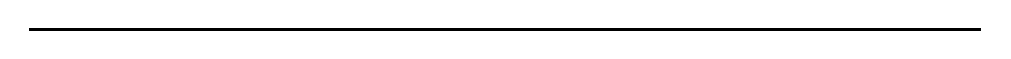
\begin{tikzpicture}
		\draw[very thick] (0,0) -- (\linewidth-\pgflinewidth,0);
	\end{tikzpicture}

	\vspace{10pt}

  \large{Dipartimento di Ingegneria Civile, Ambientale e Meccanica\\}
  \large{Corso di Laurea Magistrale in Ingegneria Civile}

  \vspace{3. cm} 

  \Huge\textsc{Tecnica delle Costruzioni\\in C.A. e Acciaio\\}
  
  \vspace{10pt}
  \Large{Progetto e verifica di elementi strutturali per un edificio intelaiato in C.A.}


  \vspace{5 cm} 
  \begin{tabular*}{\textwidth}{ l @{\extracolsep{\fill}} r }
  \Large\textsc{Studente} & \Large\textsc{Docenti}\\
  \Large{Matteo Franzoi} & \Large{Prof. Nadia Baldassino}\\
  \large{matr. 216006} & \Large{Ing. Stefano Gasperetti}\\
  \end{tabular*}

  \vspace{5cm}
    \noindent
	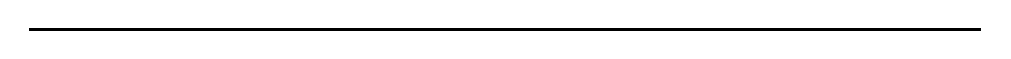
\begin{tikzpicture}
		\draw[very thick] (0,0) -- (\linewidth-\pgflinewidth,0);
	\end{tikzpicture}

 	\vspace{10pt}
    
  \Large{Anno Accademico 2019 - 2020}
  
\end{center}

\end{changegeometry}
